\documentclass[svgnames, final]{beamer} % beamer 3.10: do NOT use option hyperref={pdfpagelabels=false} !
% \documentclass[final,hyperref={pdfpagelabels=false}]{beamer} % beamer 3.07: get rid of beamer warnings
\mode<presentation> {  %% check http://www-i6.informatik.rwth-aachen.de/~dreuw/latexbeamerposter.php for examples
  \usetheme{Mizzou}    %% you should define your own theme e.g. for big headlines using your own logos 
}
\usepackage[english]{babel}
\usepackage[latin1]{inputenc}
\usepackage{amsmath,amsthm, amssymb, latexsym}
\usepackage[numbers]{natbib} %numbers instead of authoryear for [1] instead of [1980]
% \usepackage{times}\usefonttheme{professionalfonts}  % times is obsolete
\usefonttheme[onlymath]{serif}
\boldmath
 \usepackage[orientation=landscape,size=a0,scale=1.4,debug]{beamerposter}
% \usepackage[orientation=portrait,size=a0,scale=1.4,debug]{beamerposter}  % e.g. for DIN-A0 poster
% \usepackage[orientation=portrait,size=a1,scale=1.4,grid,debug]{beamerposter} % e.g. for DIN-A1 poster, with optional grid and debug output
% \usepackage[size=custom,width=100,height=75,scale=1.2,debug]{beamerposter} % e.g. for custom size poster
% \usepackage[orientation=portrait,size=a0,scale=1.0,printer=rwth-glossy-uv.df]{beamerposter}   % e.g. for DIN-A0 poster with rwth-glossy-uv printer check
% ...
% 
\usepackage{bm, bbm, caption}
\usepackage{tikz}
% A counter, since TikZ is not clever enough (yet) to handle
% arbitrary angle systems.
\newcount\mycount

\title{Particle Swarm Optimzation Assisted Markov Chain Monte Carlo}
\subtitle{}
\author{Matthew Simpson*, Scott Holan and Christopher Wikle}
\institute{*Postdoctoral Fellow, Department of Statistics, University of Missouri,\\[1ex]
Supported by NSF and Census under NSF grant SES-1132031, funded through NCRN.}

%%  \texttt{}

\date{May 20, 2016\\ \vskip1ex Spatial and Spatio-Temporal Design and\\ \vskip0.6ex Analysis for Official Statistics workshop\\ \vskip1ex University of Missouri}


\begin{document}
\begin{frame}{} 
  \begin{columns}[T]
    \begin{column}{0.32\textwidth}

      \begin{block}{\large Outline}
        \begin{itemize}\setlength{\itemsep0.5em}
        \item Heuristic optimization methods such as particle swarm optimization (PSO) allow for numerical optimization in higher dimensional spaces.
        \item Goal 1: develop better PSO algorithms using a tuning approach often used in MCMC algorithms.
        \item Goal 2: Use PSO to find posterior modes and use the Laplace approximation as a proposal for independent Metropolis-Hastings (IMH) and IMH within Gibbs (IMHwG) algorithms.
        \end{itemize}
      \end{block}
      \begin{block}{\large Particle swarm optimization (PSO) \citep{clerc2002particle,blum2008swarm}}
        \begin{itemize}\setlength{\itemsep0.5em}
        \item Goal: maximize $Q(\bm{\theta})$, $\bm{\theta}\in\Theta\subseteq \Re^p$.
        \item Define particles $\bm{\theta}_i\in\Theta$ with velocities $\bm{v}_i\in\Theta$, $i=1,2,\dots,n$.
        \item Define a neighborhood $\mathcal{N}_i$ of ``nearby'' particles for each particle.
        \item Evolve the position of a particle over time towards 1) its personal best ($\bm{p}_i\in\Theta$) and its neighborhood best ($\bm{g}_i\in\Theta$).
        \end{itemize}
        \vspace{1cm}
        \begin{itemize}
        \item[$\blacktriangleright$] Standard PSO evolution equations:
          \begin{align*}
            \bm{\theta}_i(t+1) &= \bm{\theta}_i(t) + \bm{v}_i(t)\\
            \bm{v}_i(t+1) & = \mbox{ inertia } + \mbox{ cognitive } + \mbox{ social }\\
                               &= \omega \bm{v}_i(t) + \phi_1 \bm{r}_{1i}(t)\circ[\bm{p}_i(t) - \bm{\theta}_i(t)] \\
                               &\phantom{= \omega \bm{v}_i(t)} \ + \phi_2 \bm{r}_{2i}(t)\circ[\bm{g}_i(t) - \bm{\theta}_i(t)]\\
            \bm{p}_i(t+1) &= \begin{cases} \bm{p}_i(t)   & \mbox{if }\  Q(\bm{p}_i(t)) \ge Q(\bm{\theta}_i(t + 1))\\
              \bm{\theta}_i(t+1) & \mbox{otherwise},
            \end{cases}\\
            \bm{g}_i(t+1) &= \arg\max_{\{\bm{p}_j(t+1)|j\in\mathcal{N}_i\}}Q(\bm{p}_j(t+1))
          \end{align*}
        \end{itemize}
        \begin{itemize}\setlength{\itemsep0.5em}
        \item Parameters: scalars $\omega$, $\phi_1$, and $\phi_2$ (good defaults known).
        \item Stochastic: $\bm{r}_{1i}(t)$ \& $\bm{r}_{2i}$ vectors of iid $U(0,1)$ r.v.'s.
        \end{itemize}
      \end{block}

      \begin{block}{\large Common neighborhoods}
        \begin{itemize}          \setlength{\itemsep0.5em}
          \item Global: each particle is a neighbor of each other particle.
          \item Ring-$k$: arrange particles in a ring; each particle has $k$ neighbors to the left and $k$ to the right.
        \end{itemize}
        \begin{figure}
          \centering
          {
            \begin{tikzpicture}[transform shape]
              % the multiplication with floats is not possible. Thus I split the loop in two.
              \foreach \number in {1,...,7}{
                % Computer angle:
                \mycount=\number
                \advance\mycount by 2
                \multiply\mycount by 45
                \advance\mycount by 0
                \node[draw,circle,inner sep=0.2cm] (N-\number) at (\the\mycount:2cm) {};
              }
              \foreach \number in {10,...,15}{
                % Computer angle:
                \mycount=\number
                \advance\mycount by 1
                \multiply\mycount by 45
                \advance\mycount by 22.5
                \node[draw,circle,inner sep=0.2cm] (N-\number) at (\the\mycount:2cm) {};
              }
              \foreach \number in {1,...,2}{
                % Computer angle:
                \mycount=\number
                \advance\mycount by 0
                \multiply\mycount by 45
                \advance\mycount by 22.5
                \node[circle,inner sep=0.2cm,fill] (N-\number) at (\the\mycount:2cm) {};
              }
              \foreach \number in {1,...,1}{
                % Computer angle:
                \mycount=\number
                \advance\mycount by 1
                \multiply\mycount by 45
                \advance\mycount by 0
                \node[draw=black,circle,inner sep=0.2cm,fill=black,label=Ring-1] (N-\number) at (\the\mycount:2cm) {};
              }
            \end{tikzpicture}
          }
          {
            \begin{tikzpicture}[transform shape]
              % the multiplication with floats is not possible. Thus I split the loop in two.
              \foreach \number in {2,...,6}{
                % Computer angle:
                \mycount=\number
                \advance\mycount by 2
                \multiply\mycount by 45
                \advance\mycount by 0
                \node[draw,circle,inner sep=0.2cm] (N-\number) at (\the\mycount:2cm) {};
              }
              \foreach \number in {10,...,15}{
                % Computer angle:
                \mycount=\number
                \advance\mycount by 1
                \multiply\mycount by 45
                \advance\mycount by 22.5
                \node[draw,circle,inner sep=0.2cm] (N-\number) at (\the\mycount:2cm) {};
              }
              \foreach \number in {1,...,2}{
                % Computer angle:
                \mycount=\number
                \advance\mycount by 0
                \multiply\mycount by 45
                \advance\mycount by 22.5
                \node[circle,inner sep=0.2cm,fill] (N-\number) at (\the\mycount:2cm) {};
              }
              \foreach \number in {1,...,3}{
                % Computer angle:
                \mycount=\number
                \advance\mycount by 0
                \multiply\mycount by 45
                \advance\mycount by 0
                \node[circle,inner sep=0.2cm,fill] (N-\number) at (\the\mycount:2cm) {};
              }
              \foreach \number in {1,...,1}{
                % Computer angle:
                \mycount=\number
                \advance\mycount by 1
                \multiply\mycount by 45
                \advance\mycount by 0
                \node[draw=black,circle,inner sep=0.2cm,fill=black,label=Ring-2] (N-\number) at (\the\mycount:2cm) {};
              }
            \end{tikzpicture}
          }
          {
            \begin{tikzpicture}[transform shape]
              % the multiplication with floats is not possible. Thus I split the loop in two.
              \foreach \number in {2,...,6}{
                % Computer angle:
                \mycount=\number
                \advance\mycount by 2
                \multiply\mycount by 45
                \advance\mycount by 0
                \node[draw,circle,inner sep=0.2cm] (N-\number) at (\the\mycount:2cm) {};
              }
              \foreach \number in {10,...,15}{
                % Computer angle:
                \mycount=\number
                \advance\mycount by 1
                \multiply\mycount by 45
                \advance\mycount by 22.5
                \node[draw,circle,inner sep=0.2cm] (N-\number) at (\the\mycount:2cm) {};
              }
              \foreach \number in {1,...,4}{
                % Computer angle:
                \mycount=\number
                \advance\mycount by -1
                \multiply\mycount by 45
                \advance\mycount by 22.5
                \node[circle,inner sep=0.2cm,fill] (N-\number) at (\the\mycount:2cm) {};
              }
              \foreach \number in {1,...,3}{
                % Computer angle:
                \mycount=\number
                \advance\mycount by 0
                \multiply\mycount by 45
                \advance\mycount by 0
                \node[circle,inner sep=0.2cm,fill] (N-\number) at (\the\mycount:2cm) {};
              }
              \foreach \number in {1,...,1}{
                % Computer angle:
                \mycount=\number
                \advance\mycount by 1
                \multiply\mycount by 45
                \advance\mycount by 0
                \node[draw=black,circle,inner sep=0.2cm,fill=black,label=Ring-3] (N-\number) at (\the\mycount:2cm) {};
              }
            \end{tikzpicture}
          }
          {
            \begin{tikzpicture}[transform shape]
              % the multiplication with floats is not possible. Thus I split the loop in two.
              \foreach \number in {2,...,8}{
                % Computer angle:
                \mycount=\number
                \advance\mycount by 1
                \multiply\mycount by 45
                \advance\mycount by 0
                \node[draw,circle,inner sep=0.2cm,fill] (N-\number) at (\the\mycount:2cm) {};
              }
              \foreach \number in {9,...,16}{
                % Computer angle:
                \mycount=\number
                \advance\mycount by 1
                \multiply\mycount by 45
                \advance\mycount by 22.5
                \node[draw,circle,inner sep=0.2cm,fill] (N-\number) at (\the\mycount:2cm) {};
              }
              \foreach \number in {1,...,1}{
                % Computer angle:
                \mycount=\number
                \advance\mycount by 1
                \multiply\mycount by 45
                \advance\mycount by 0
                \node[draw=black,circle,inner sep=0.2cm,fill=black,label=Global] (N-\number) at (\the\mycount:2cm) {};
              }
            \end{tikzpicture}
          }
          \caption*{Filled in white particles are neighbors of the filled in black particle.}
        \end{figure}
         
      \end{block}
      \vfill
    \end{column}
    
    \begin{column}{0.32\textwidth}
      \vfill
      \begin{block}{\large Bare Bones PSO (BBPSO) \citep{kennedy2003bare}}
        \begin{itemize}
        \item[$\blacktriangleright$] Simplify by removing the velocity term:
          \begin{align}\label{eq:bbpso}
            \theta_{ij}(t+1) \sim N\left(\frac{p_{ij}(t) + g_{ij}(t)}{2}, |p_{ij}(t) - g_{ij}(t)|\right)
          \end{align}
          for $j=1,2,\dots,p$. Updates for $\bm{p}_i$ and $\bm{g}_i$ as in PSO.
        \end{itemize}
        \vspace{1cm}
        \begin{itemize}
          \setlength{\itemsep0.5em}
        \item BBPSO variants:
          \begin{itemize}
            \setlength{\itemsep0.5em}
          \item BBPSOxp: every iteration $\theta_{ij}(t+1)$ has 50\% chance of moving according to \eqref{eq:bbpso} and a 50\% chance of moving to $g_{ij}(t)$ \citep{kennedy2003bare}.
          \item BBPSO-MC: same as \eqref{eq:bbpso} except any particle currently at its neighborhood best moves according to
            \begin{align*}
              \theta_{ij}(t+1) = p_{i_1j}(t) + 0.5(p_{i_2j}(t) - p_{i_3j}(t))
            \end{align*}
            where $i_1$, $i_2$, and $i_3$ are distinct, randomly selected particles \cite{zhang2011novel}.
          \item BBPSOxp-MC: combine both.
          \end{itemize}
        \end{itemize}
        \vspace{1cm}
      \end{block}
      \vfill
      \begin{block}{\large Adaptively tuned BBPSO (AT-BBPSO)}
        \begin{itemize}
        \item[$\blacktriangleright$] Add scale parameter to BBPSO and tune it (tuned version of \citep{hsieh2010modified}):
          \begin{align*}
            \theta_{ij}(t+1) &\sim T_{df}\left(\frac{p_{ij}(t) + g_{ij}(t)}{2}, |p_{ij}(t) - g_{ij}(t)|e^{\lambda(t)}\right)\\
                             &\mbox{ for } j=1,2,\dots,p\\
            R(t+1) &= \#\{\bm{p}_i(t+1)\neq \bm{p}_i(t): i=1,2,\dots,n\}/n\\
            \lambda(t+1) &= \lambda(t) + 0.1\times sgn(R(t+1) - R^*)
          \end{align*}
        \end{itemize}
        \begin{itemize} 
          \setlength{\itemsep0.5em}
        \item The target acceptance rate $R^*$ roughly controls exploitation vs. exploration. $R^* = 0.2$ or $0.3$ seems to work well --- similar to a random walk Metropolis acceptance rate.
        \item The degrees of freedom parameter $df$ is harder to interpret, but generally small is good. E.g. $df=1$ or $df=3$.
        \item AT-BBPSOxp-MC w/ Ring-1 \& above settings often works well.
        \end{itemize}
      \end{block}
      \vfill
      \begin{block}{\large Spatially smoothing ACS county population estimates}
        \begin{itemize}\setlength{\itemsep0.5em}
        \item Data model: $z_k \sim Pois\left(e^{\bm{x}_k'\bm{\beta} + \bm{s}_k'\bm{\delta}}\right)$;\ \ \ \ \  Fixed effects: $\bm{x}_k' = 1$.
        \item Random effects: $\bm{s}_k':1\times r$ from truncated Moran's I basis \citep{hughes2013dimension,porter2015bayesian}.
        \item IID model: $\bm{\delta} \sim N(0,\sigma^2\bm{\mathrm{I}})$; \ \ \ Full model: $\bm{\delta} \sim N(\bm{0}, \bm{\Sigma})$.
        \end{itemize}
        \begin{figure}
          \centering
          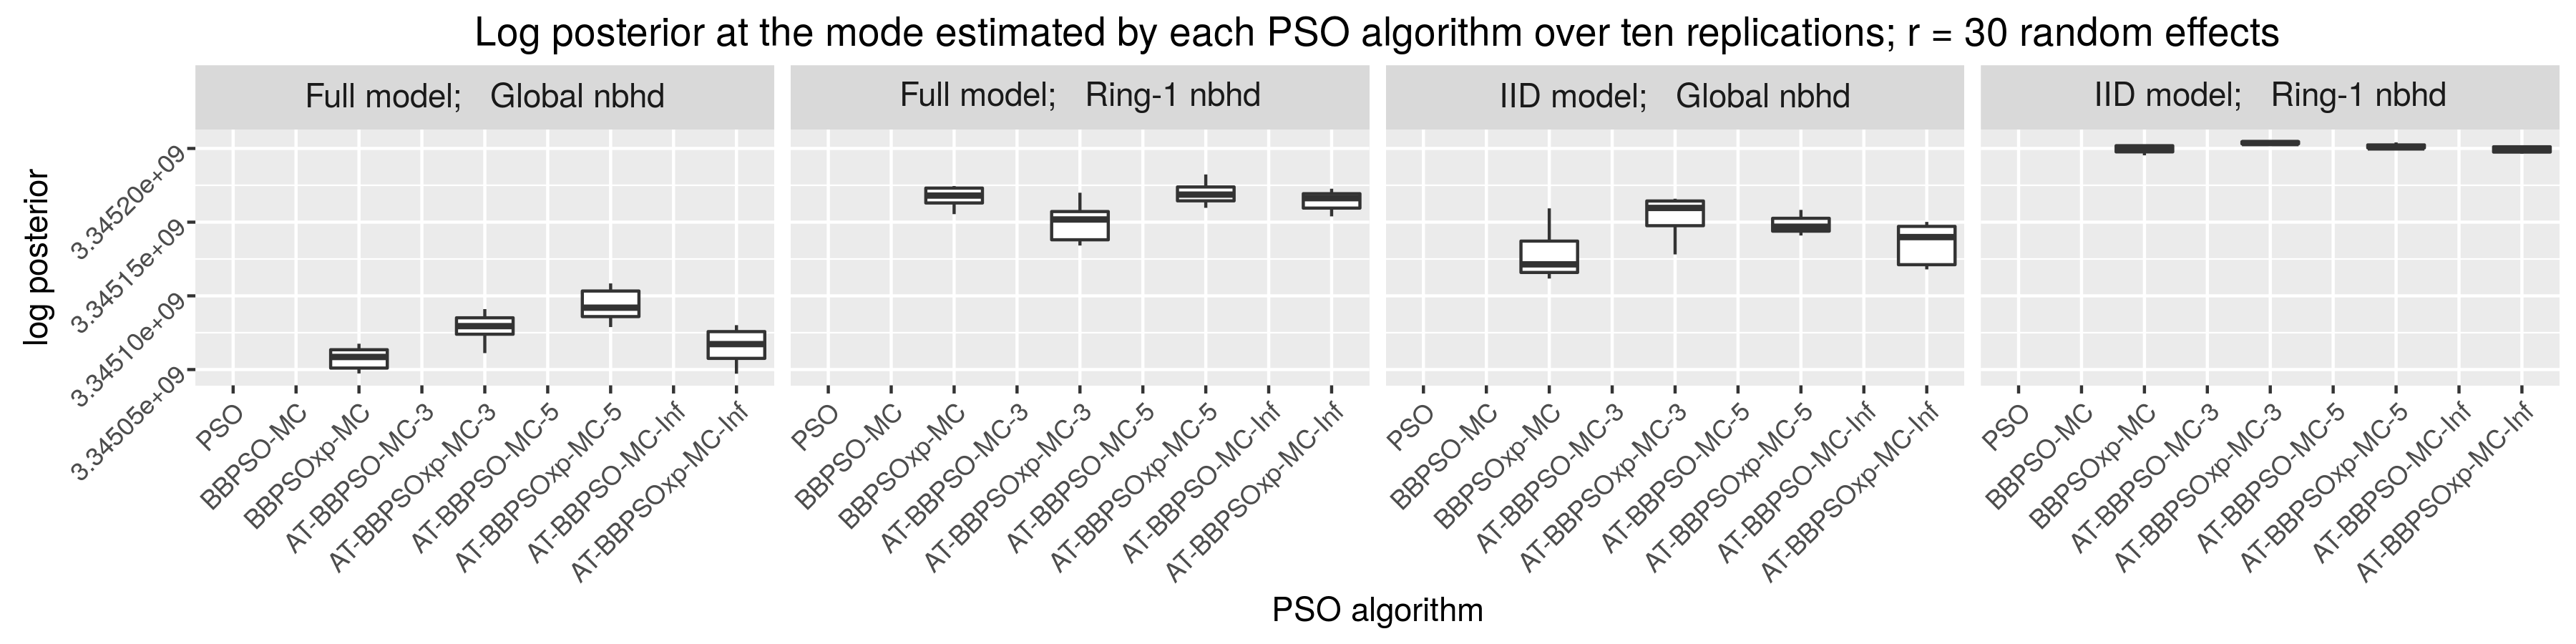
\includegraphics[scale=1]{../pop/maxplotpost.png}
        \end{figure}
        \end{block}
    \end{column}

    \begin{column}{0.32\textwidth}
      \vfill
      \begin{block}{\large MCMC Algorithms}
        \begin{itemize}\setlength{\itemsep0.5em}
        \item PSO-IMH: find posterior mode via PSO and use Laplace approximation as a proposal (a $T_\nu$ distribution).
        \item PSO-IMH within Gibbs (PSO-IMHwG): 
          \begin{itemize}\setlength{\itemsep0.5em}
          \item Conditionally conjugate step for $\bm{\Sigma}$ or $\sigma^2$.
          \item IMH for $(\bm{\beta}, \bm{\delta})$ using conditional distribution implied by $T_\nu$ approximation to the full posterior as a proposal (obtained via PSO).
          \end{itemize}
 %       \item Single move RW within Gibbs (RWwG) w/ conjugate draw for $\bm{\Sigma}$ or $\sigma^2$.
        \item Block RW within Gibbs (B-RWwG) w/ conjugate draw for $\bm{\Sigma}$ or $\sigma^2$.
 %        \item IMH within Gibbs (IMHwG) w/ proposal for $(\bm{\beta}, \bm{\delta})$ from prior. 
        \end{itemize}
        \vfill
        \begin{itemize}
        \item[$\blacktriangleright$] $\nu$: degrees of freedom in $T_\nu$ proposal for PSO-IMH and PSO-IMHwG.
          \begin{itemize}\setlength{\itemsep0.5em}
          \item Choose to optimize the Metropolis acceptance rate.
          \item For these models, $\nu=\infty$ --- i.e. a Gaussian proposal.
          \end{itemize}
        \end{itemize}
      \end{block}
      \vfill
      \begin{block}{\large MCMC Results}
        \begin{table}[ht]
          \centering
          \begin{tabular}{|l|rrrr|rrrr|}
            \multicolumn{2}{c}{IID Model} & \multicolumn{7}{c}{}\\
            \multicolumn{1}{c}{} &\multicolumn{4}{c}{$n_{eff}$}&\multicolumn{4}{c}{time/$n_{eff}$}\\
            \hline
            r  & IMH & IMHwG & RWwG & B-RWwG & IMH & IMHwG & RWwG & B-RWwG \\ 
            \hline
            10 & 23170 & 46177 & 8072 & 1168 & 24 & 23 & 201 & 146 \\ 
            20 & 16958 & 43005 & 5739 & 646 & 27 & 26 & 506 & 215 \\ 
            30 & 30237 & 39739 & 4440 & 404 & 16 & 24 & 790 & 483 \\ 
            \hline
            \multicolumn{9}{c}{}\\
            \multicolumn{2}{c}{Full Model} & \multicolumn{7}{c}{}\\
            \multicolumn{1}{c}{} &\multicolumn{4}{c}{$n_{eff}$}&\multicolumn{4}{c}{time/$n_{eff}$}\\
            \hline
            r & IMH & IMHwG & RWwG & B-RWwG & IMH & IMHwG & RWwG & B-RWwG \\ 
            \hline
            5 & 32 & 47240 & 8089 & 2070 & 14433 & 21 & 131 & 170 \\ 
            7 & 37 & 42459 & 7811 & 1743 & 11188 & 20 & 145 & 167 \\ 
            9 & 9 & 717 & 8298 & 1417 & 32197 & 876 & 126 & 153 \\ 
            \hline
          \end{tabular}
          \caption*{Effective sample size ($n_{eff}$) and time in seconds per 10,000 effective samples (time$/n_{eff}$) for each algorithm in both models with various numbers of random effects ($r$). IMH algorithms with tiny acceptance rates are indicated by a ``---''.}
        \end{table}
        \begin{itemize}\setlength{\itemsep0.5em}
          \item In the IID model the log variance is approximately normal\\ $\implies$ PSO-IMH algorithms work well.
          \item In the Full model we only have one ``observation'' with covariance $\bm{\Sigma}$\\ $\implies$ normal approximation is bad \& PSO-IMH works poorly.
        \end{itemize}
      \end{block}
      \vfill
      \begin{block}{\large References}
        {\tiny
          \nocite{*} % Print all references regardless of whether they were cited in the poster or not
          \bibliographystyle{apalike} % Plain referencing style
          \bibliography{psopost} % Use the example bibliography file sample.bib
        }
      \end{block}
      \vfill
    \end{column}
  \end{columns}
\end{frame}
\end{document}
